\section{Interface utilisateur}

Nous avons opt� pour une interface simple en mode graphique.
Pour cela, nous avons utiliser la librairie QT.
Notre interface poss�de
\begin{itemize}
\item un menu qui permet d'ouvrir un fichier image (gr�ce � un popup menu)
\item une liste contenant les images charg�es, permettant ainsi un acc�s
rapide.\\ Cette liste ne repr�sente pas les objets contenus dans le
cache. Ces derniers sont affich�s dans le terminal.
\item une zone r�serv�e � l'affichage de l'image
\end{itemize}

Le visualisateur a besoin d'un type QImage. Ce dernier est
pass� comme template au Loader qui peut ainsi cr�er une image correct.\\\\

\begin{figure}[!htp]
  \label{interface}
    \begin{center}
      	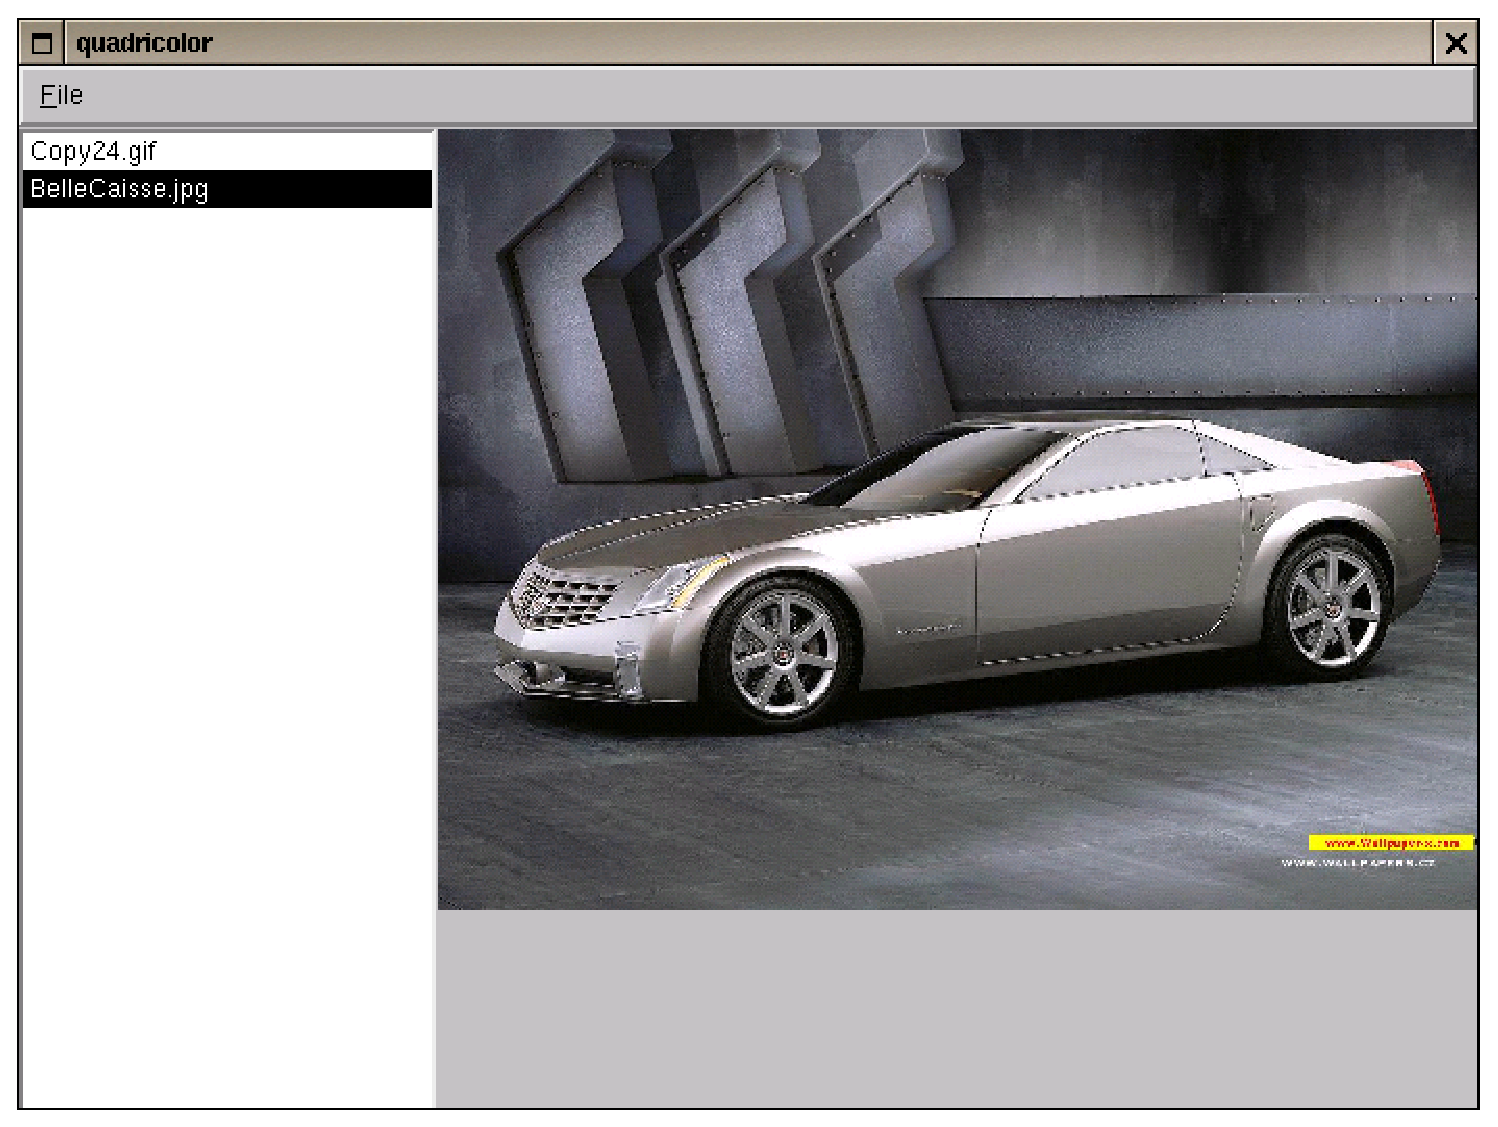
\includegraphics[width=13cm, height=8cm]{view.eps}
      \caption[Capture d'�cran]{L'interface utilisateur}
    \end{center}
\end{figure}	


